%==============================================================

\chapter{Results}\label{bds2}

Very small 100 Song Dataset plus 20 Cover Songs to evaluate and compare similarity metrics. Full similarity matrices. 
High performance/ throughput tests with full 12000 song testset to evaluate full load performance.\\

\section{Runtime}

\section{feature separation quality}

\textit{\textbf{Which features are useful, which not (looking at you rhythm histogram)\\}}
\\
\noindent correlation of features in figure \ref{fig:corr}\\
\begin{figure}[htbp]
	\centering
	\framebox{\parbox{1\textwidth}{ 			
			\begin{subfigure}{.495\textwidth}
				\centering    
				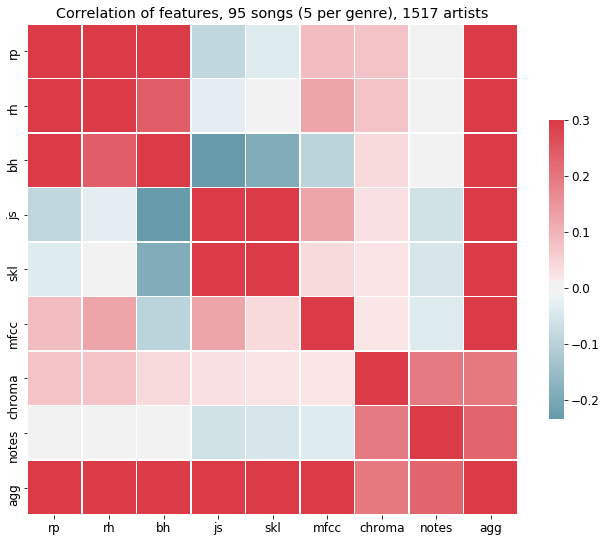
\includegraphics[scale=0.35]{Images/SparkFeat/correlation1517_95.png}
				\caption{95 songs from 19 genres, 1517 artists}
				\label{cor1}
			\end{subfigure}		
			\begin{subfigure}{.495\textwidth}
				\centering     
				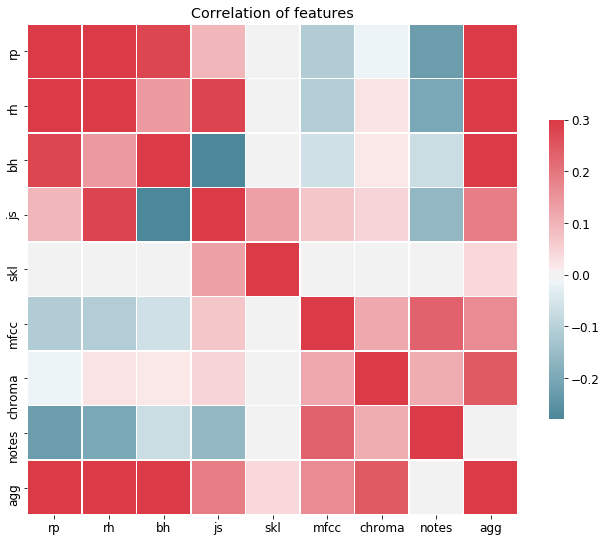
\includegraphics[scale=0.35]{Images/SparkFeat/correlation10.png}
				\caption{10 songs from 4 genres, full ds}
				\label{cor2}
			\end{subfigure}%		
	}}
	\caption{correlation of features}
	\label{fig:corr}
\end{figure}
\FloatBarrier

correlation of features in figure \ref{fig:corr2}\\
\begin{figure}[htbp]
	\centering
	\framebox{\parbox{1\textwidth}{ 			
			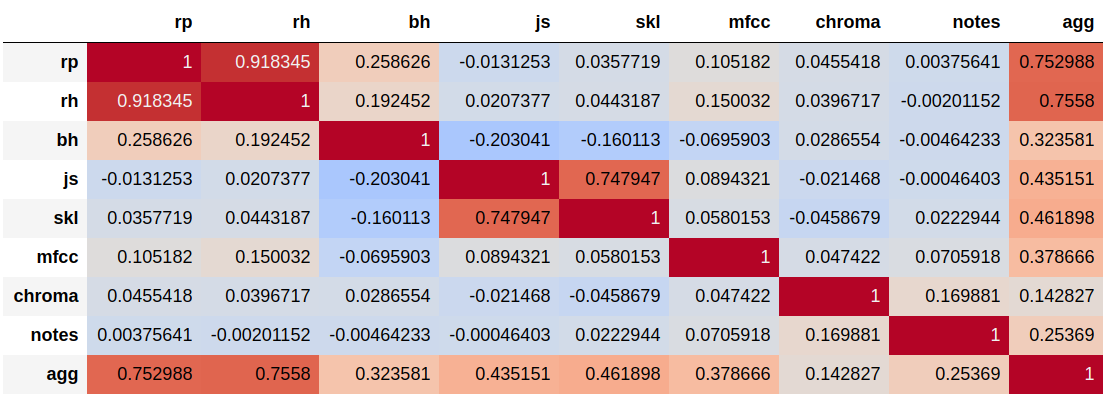
\includegraphics[scale=0.33]{Images/SparkFeat/corr_95_1517.png}	
	}}
	\caption{correlation 95 songs, 19 genres (5 each), 1517 artists}
	\label{fig:corr2}
\end{figure}
\FloatBarrier

\noindent Scatter Matrix, 5 songs of each genre from 1517 artists - distances combined, main diagonal = Kernel Density Estimation in figure \ref{fig:corr3}
\begin{figure}[htbp]
	\centering
	\framebox{\parbox{1\textwidth}{ 			
			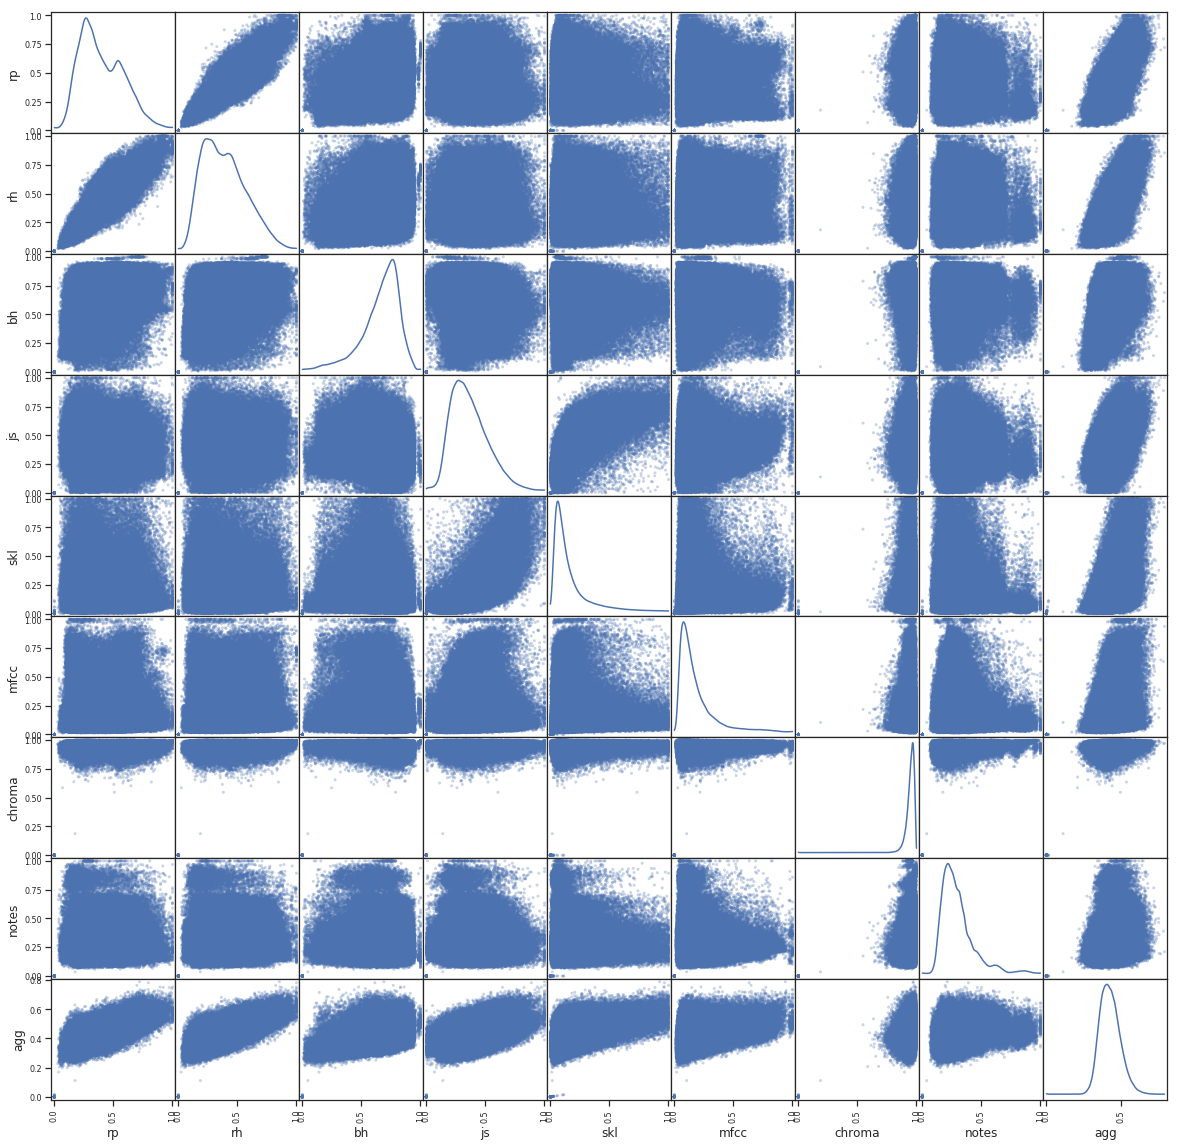
\includegraphics[scale=0.36]{Images/SparkFeat/scatter1517_KernelDensityEstimationHD.png}	
	}}
	\caption{correlation 95 songs, 19 genres (5 each), 1517 artists}
	\label{fig:corr3}
\end{figure}
\FloatBarrier

\noindent Scatter Matrix, 1 Song (New Age) from 1517 artists - distances, main diagonal = Histogram, all genres in figure \ref{fig:corr4}
\begin{figure}[htbp]
	\centering
	\framebox{\parbox{1\textwidth}{ 			
			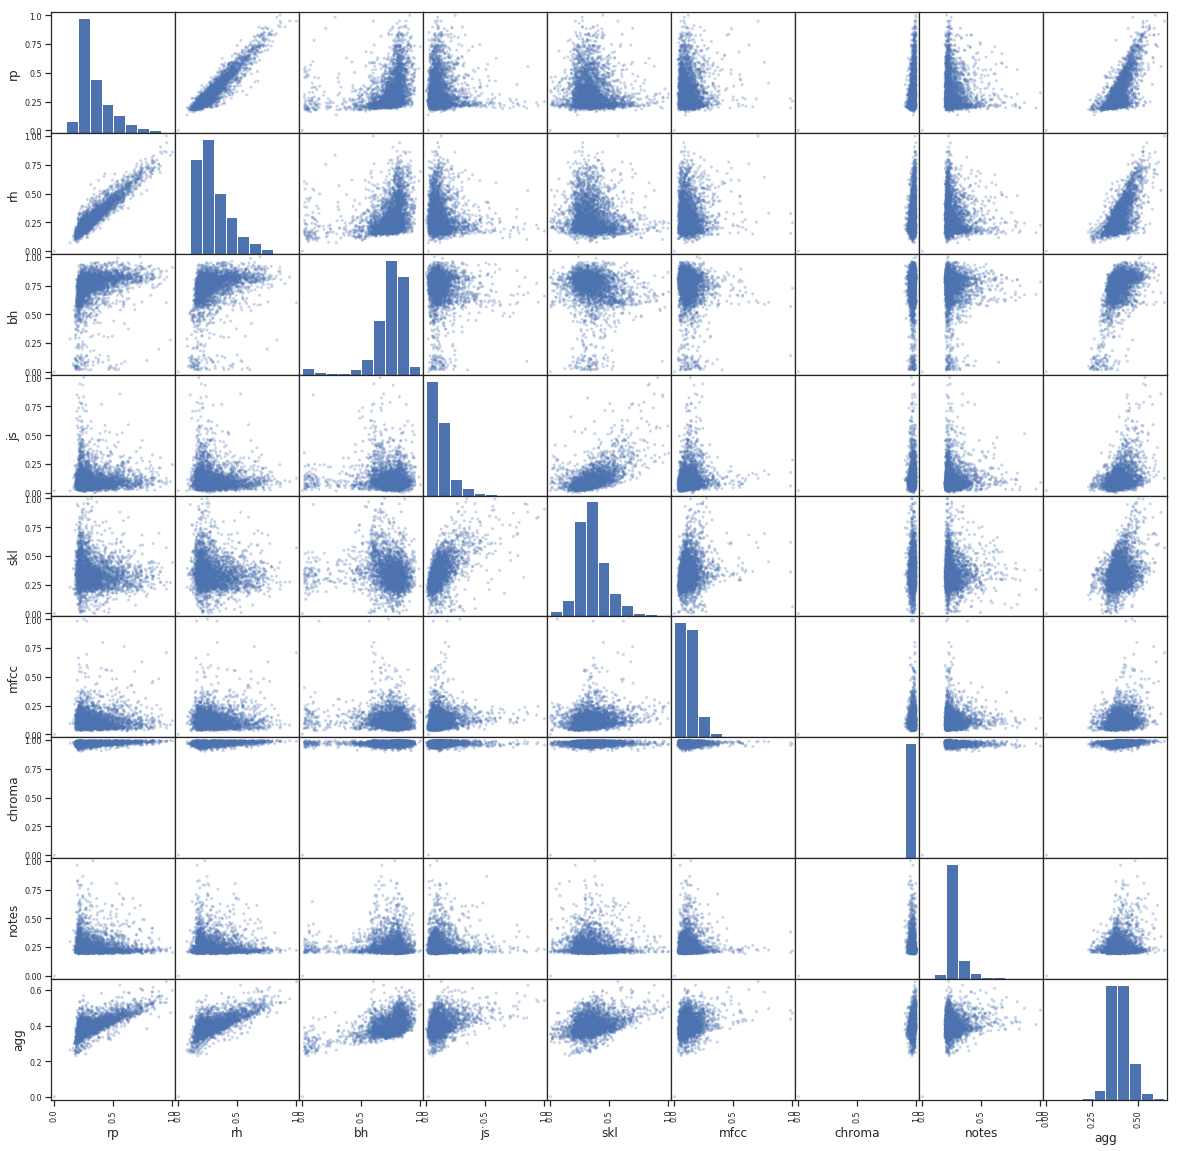
\includegraphics[scale=0.36]{Images/SparkFeat/scatter1517_singlesongHistogramHD.png}	
	}}
	\caption{distances 1 song, New Age, 1517 artists}
	\label{fig:corr4}
\end{figure}
\FloatBarrier

\noindent Scatter Matrix, 1 Song (Rock/ Metal) from 1517 artists - distances, main diagonal = Kernel Density Estimation, picked subset of 3 genres\\ All features combined recommends Rock primarily\\
Most interesting Detail: Plot JS - RP: overall similarity JS between Rock and Hip Hop - overall similarity RP between Classical and Metal - only one feature would not be able to separate all 3 genres in figure \ref{fig:corr5}
\begin{figure}[htbp]
	\centering
	\framebox{\parbox{1\textwidth}{ 			
			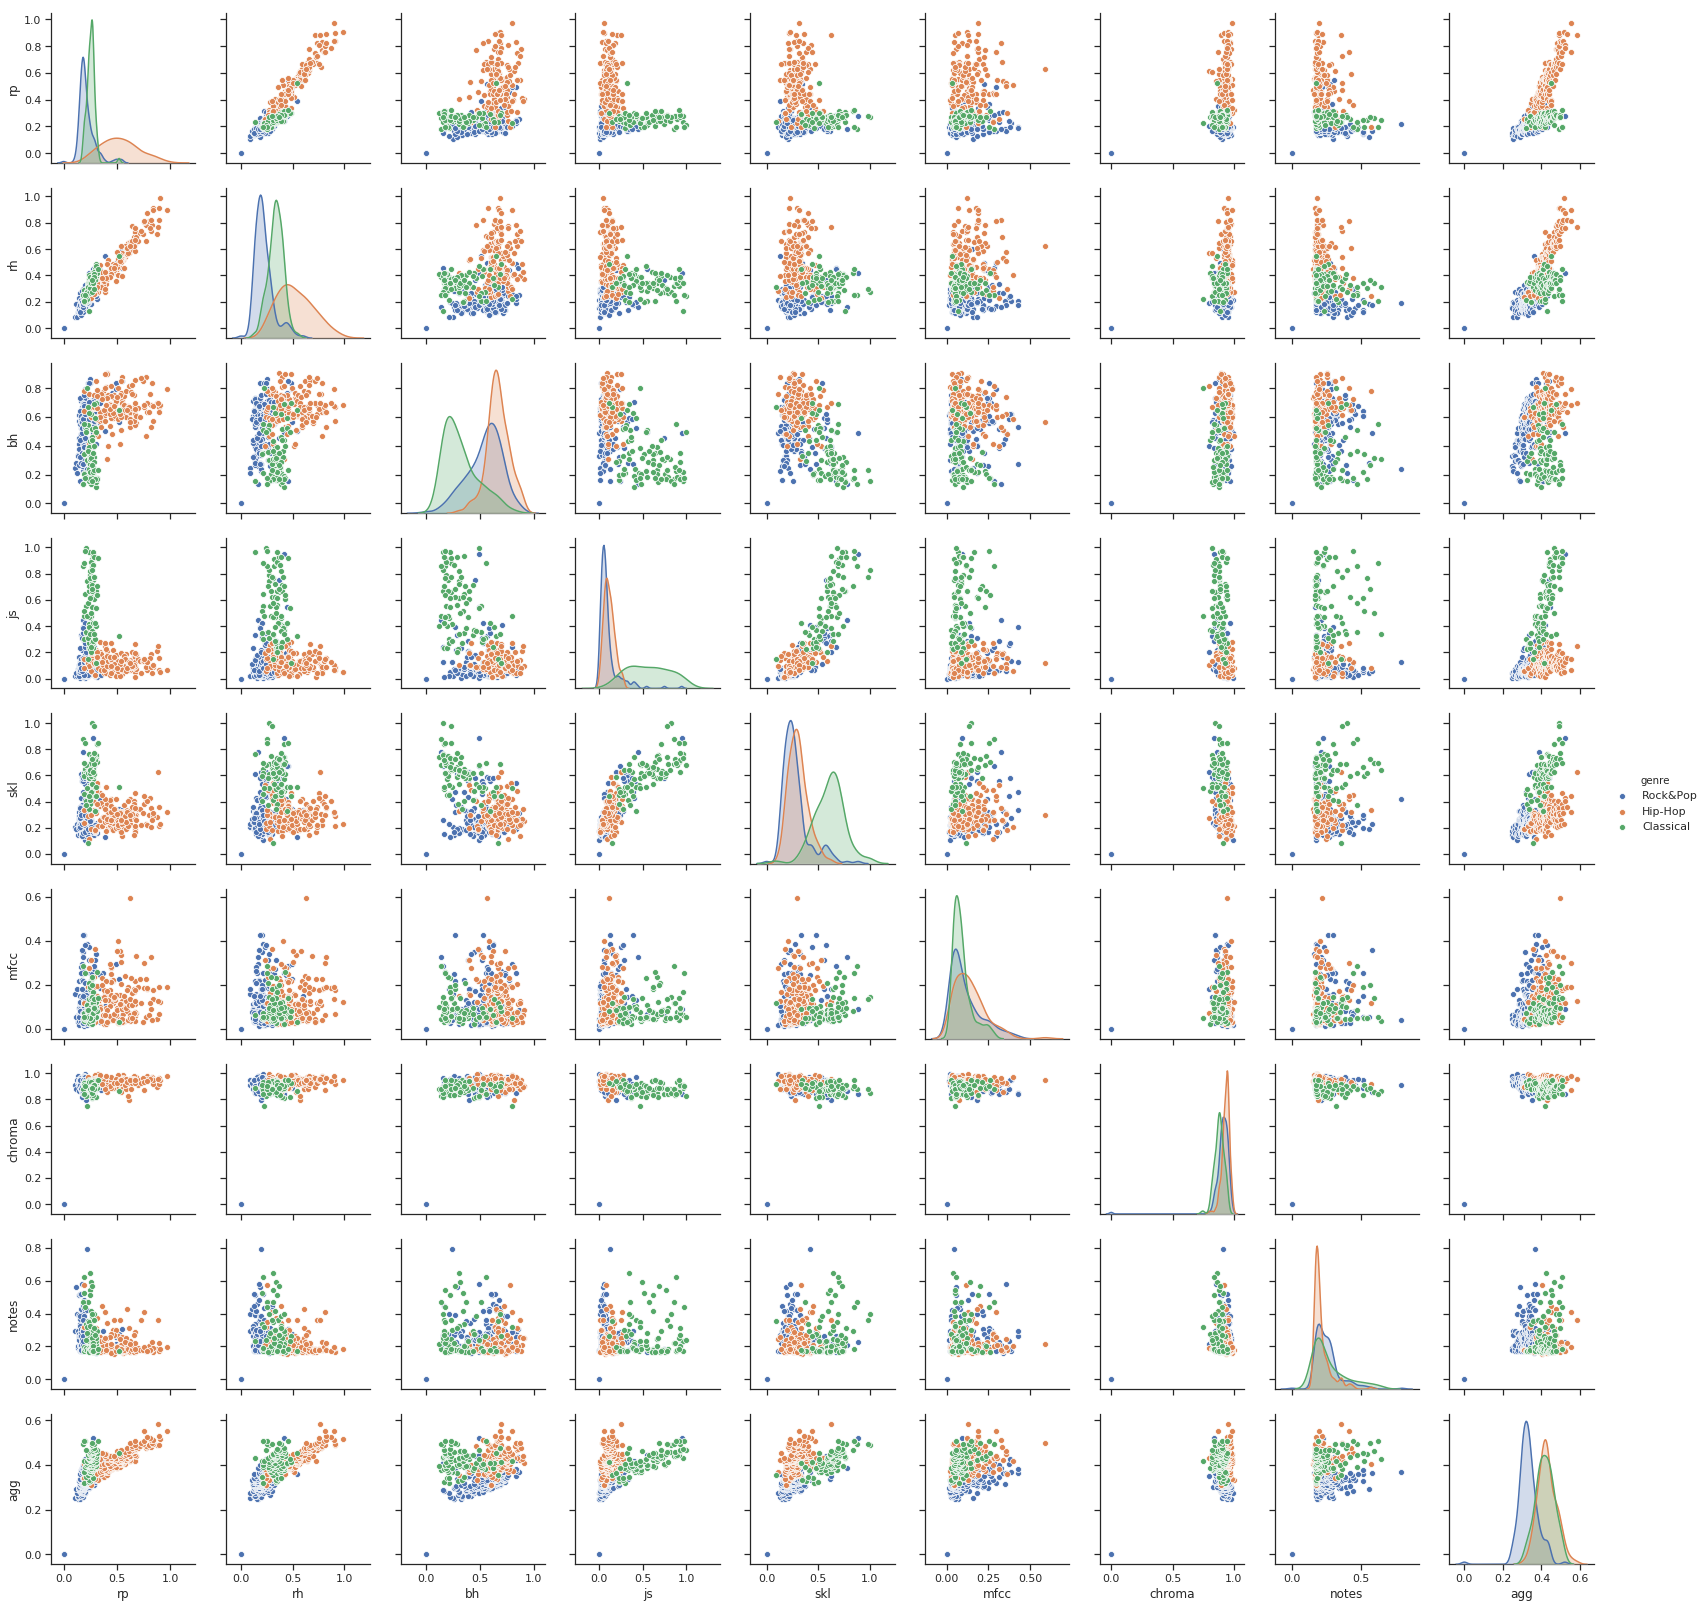
\includegraphics[scale=0.25]{Images/SparkFeat/scatter1517_singlesongHDrock.png}	
	}}
	\caption{distances 1 song, Rock/ Metal, 1517 artists, 3 genres}
	\label{fig:corr5}
\end{figure}
\FloatBarrier

\noindent Scatter Matrix, 1 Song (New Age) from 1517 artists - distances, main diagonal = Kernel Density Estimation,all genres in figure\\
No combination of features is able to accurately separate New Age from Rock and Pop\ref{fig:corr6}
\begin{figure}[htbp]
	\centering
	\framebox{\parbox{1\textwidth}{ 			
			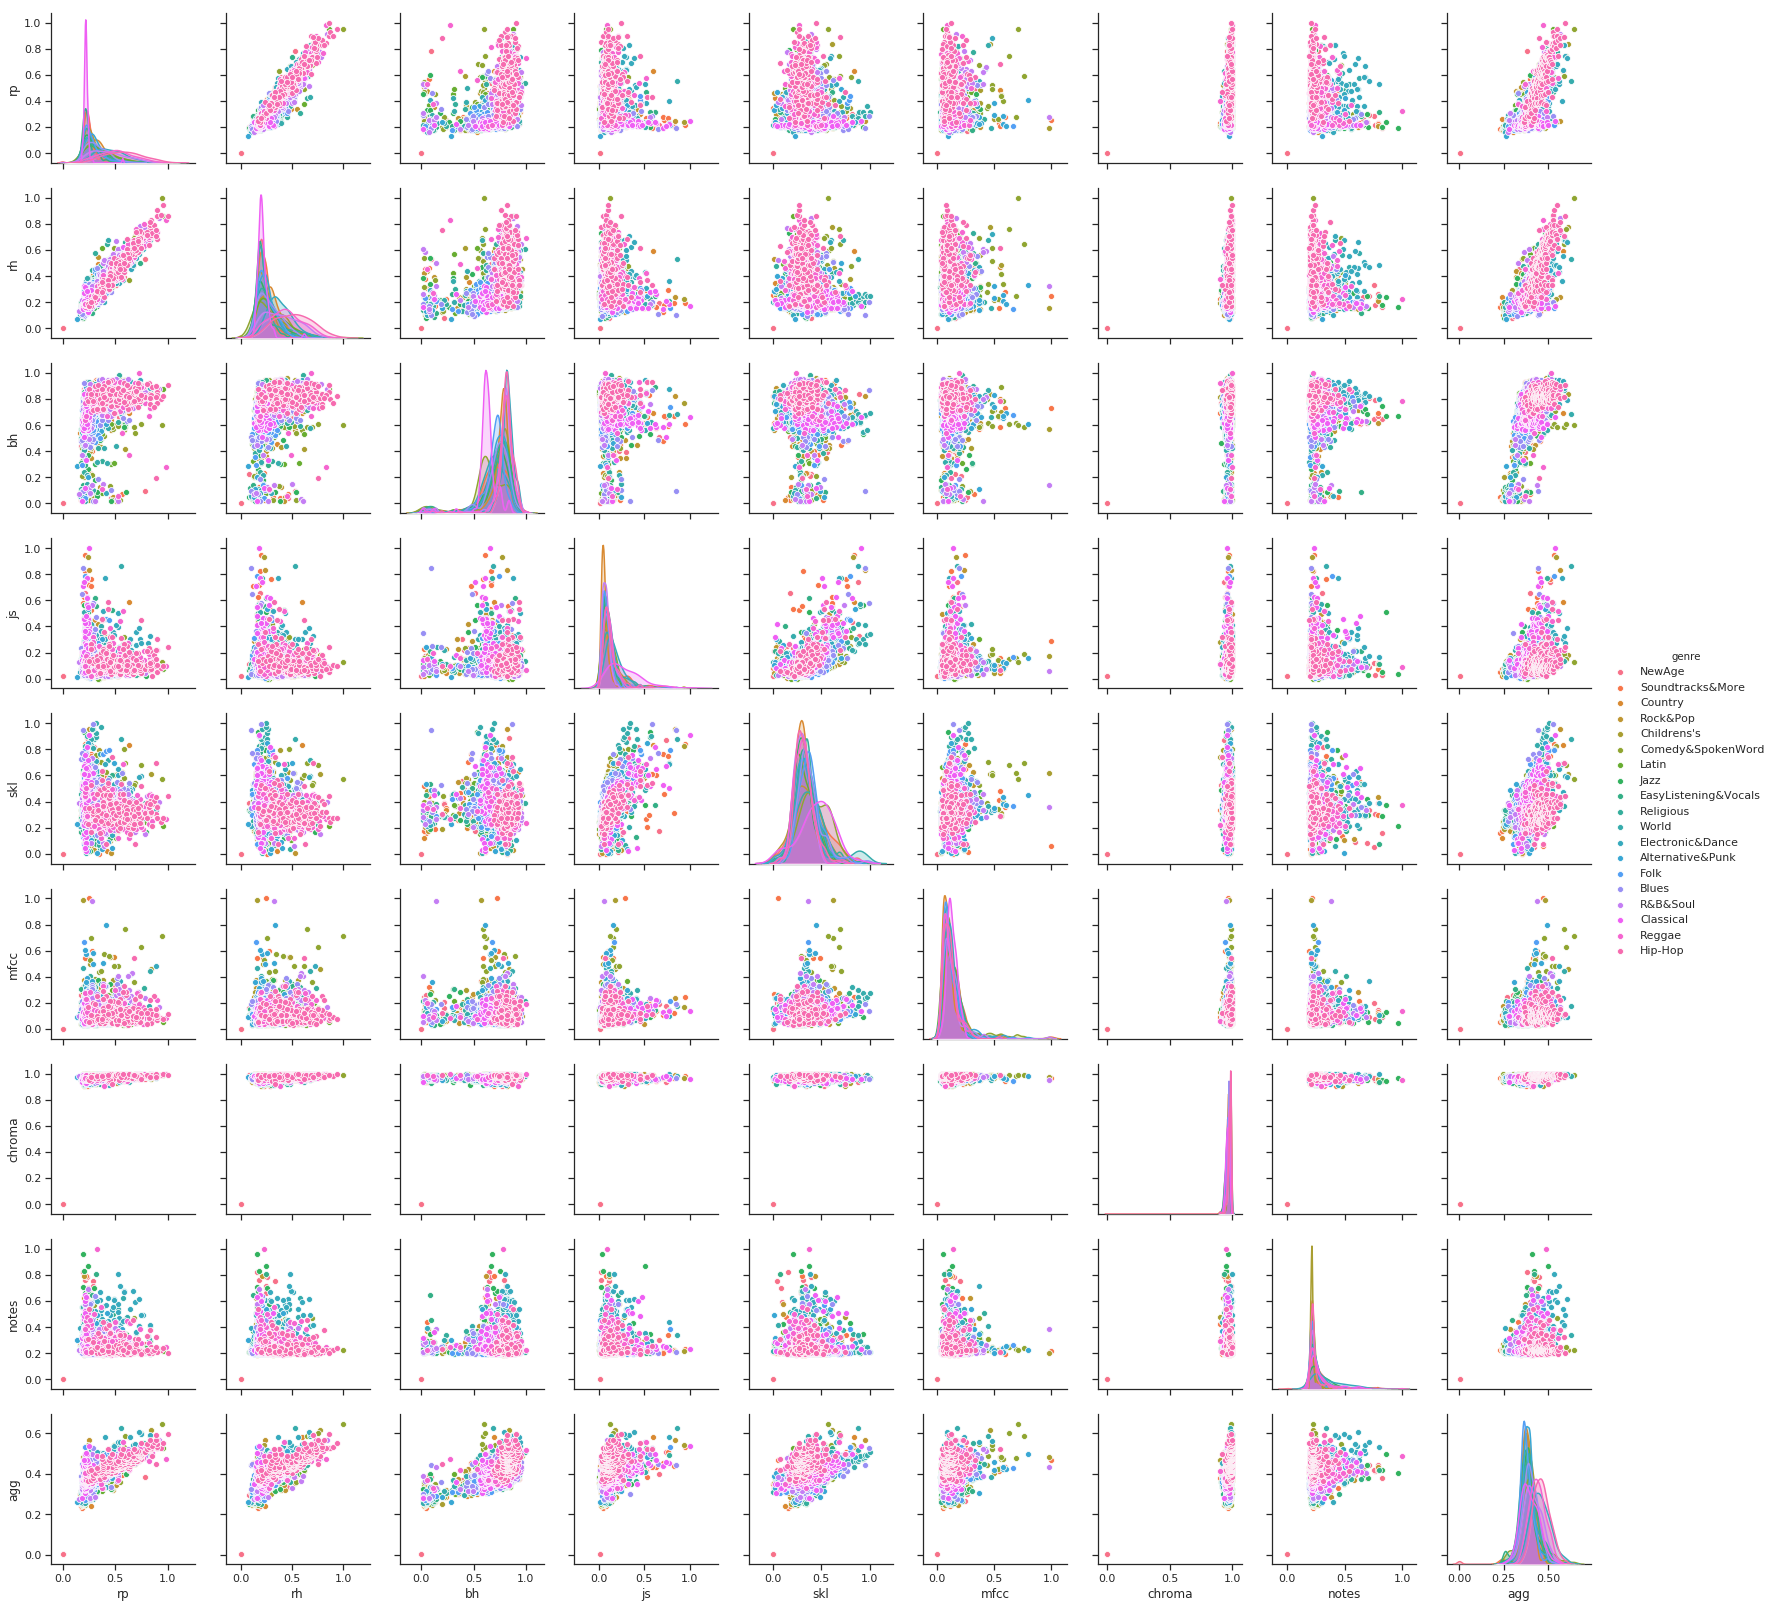
\includegraphics[scale=0.25]{Images/SparkFeat/scatter1517_singlesongHD.png}	
	}}
	\caption{distances 1 song, New Age, 1517 artists, all genres}
	\label{fig:corr6}
\end{figure}
\FloatBarrier

\noindent Scatter Matrix, 1 Song (Classics) from 100 song sample - distances, main diagonal = Kernel Density Estimation, picked subset of 4 genres in figure \ref{fig:corr7}
\begin{figure}[htbp]
	\centering
	\framebox{\parbox{1\textwidth}{ 			
			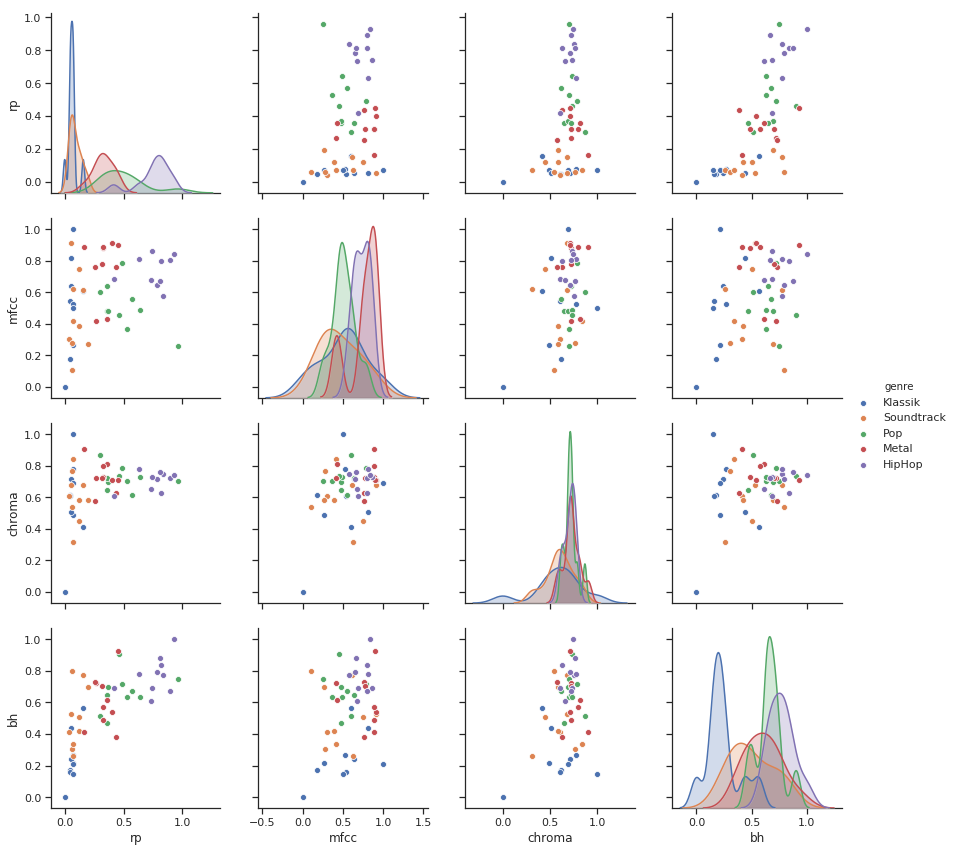
\includegraphics[scale=0.45]{Images/SparkFeat/scatter100_1classicsong.png}	
	}}
	\caption{distances 1 song (Classical), 4 genres (10 songs each)}
	\label{fig:corr7}
\end{figure}
\FloatBarrier

\noindent distances from classical song out of 1517 artists dataset in figure \ref{fig:featsep}\\

\begin{figure}[htbp]
	\centering
	\framebox{\parbox{1\textwidth}{ 			
			\begin{subfigure}{.495\textwidth}
				\centering    
				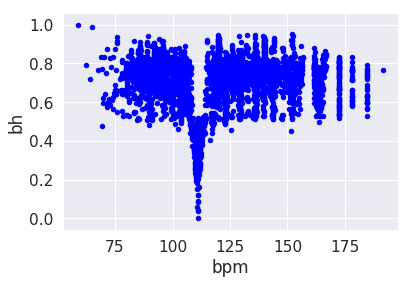
\includegraphics[scale=0.3]{Images/SparkFeat/BH_BPM.png}
				\caption{Beat Histogram vs BPM}
				\label{fs1}
			\end{subfigure}		
			\begin{subfigure}{.495\textwidth}
				\centering     
				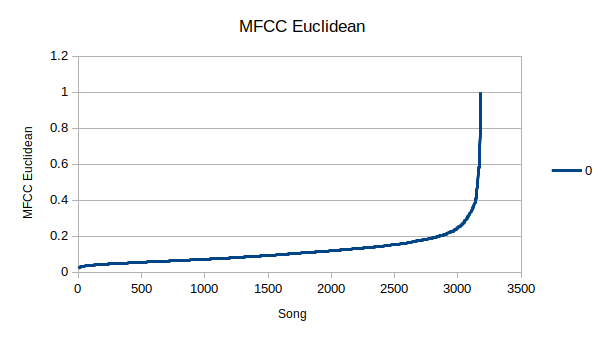
\includegraphics[scale=0.5]{Images/SparkFeat/MFCC_Eucl.png}
				\caption{MFCC Euclidean}
				\label{fs2}
			\end{subfigure}%	
			
			\begin{subfigure}{.495\textwidth}
				\centering    
				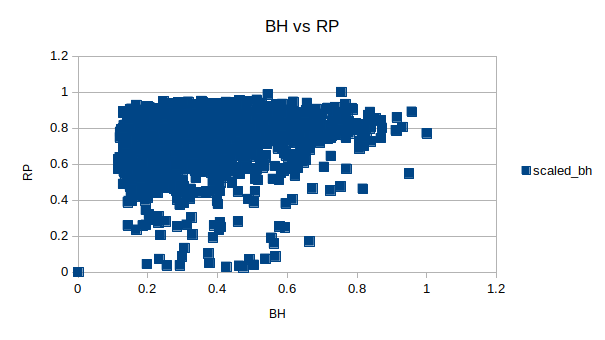
\includegraphics[scale=0.5]{Images/SparkFeat/BH_RP.png}
				\caption{Beat Histogram vs Rhythm Patterns}
				\label{fs3}
			\end{subfigure}
			\begin{subfigure}{.495\textwidth}
				\centering     
				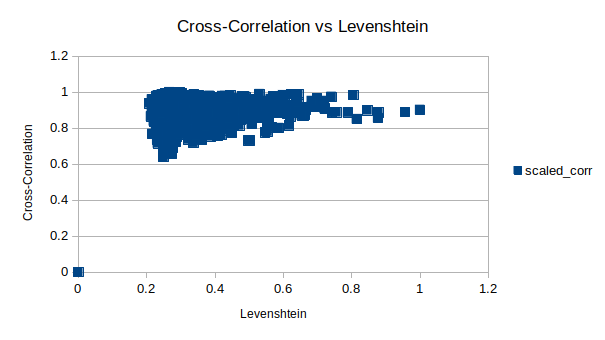
\includegraphics[scale=0.5]{Images/SparkFeat/Cross-Corr_Levenshtein.png}
				\caption{Cross-correlation vs Levenshtein}
				\label{fs4}
			\end{subfigure}%		
	}}
	\caption{genre recall 100 songs}
	\label{fig:featsep}
\end{figure}
\FloatBarrier

\section{Cover song identification}

\textit{\textbf{Able to find "Rock you like a Hurricane" cover as top recommendation in over 11500 songs\\}}
\ \\
\textit{\textbf{counting the hits in the top 10 results of 80 requested songs on 164 song dataset covers80:\\}}
\begin{itemize}
	\item chroma: 16
	\item notes: 24
	\item chroma + notes: 24
	\item notes + rp: 22
	\item chroma + notes + rp: 28
	\item mfcc + notes + rp: 20
\end{itemize}
\textit{interesting sidenote: results of chroma only and notes only different! Nearly ever}

\section{Genre similarity}

\textbf{\textit{\underline{100 Song Testset, 10 genres:\\}}} 
\begin{figure}[htbp]
	\centering
	\framebox{\parbox{1\textwidth}{ 			
			\begin{subfigure}{.495\textwidth}
				\centering    
				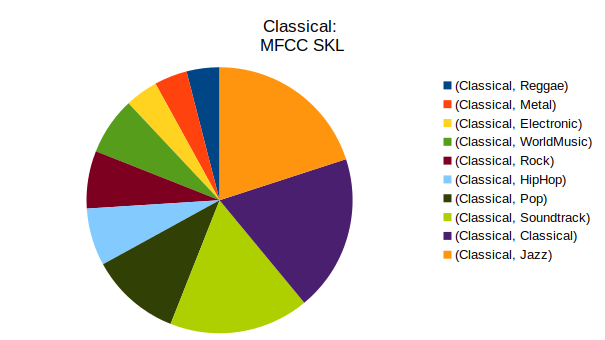
\includegraphics[scale=0.3]{Images/SparkFeat/Classical_MFCC_SKL.png}
				\caption{Classical MFCC SKL}
				\label{cms}
			\end{subfigure}		
			\begin{subfigure}{.495\textwidth}
				\centering     
				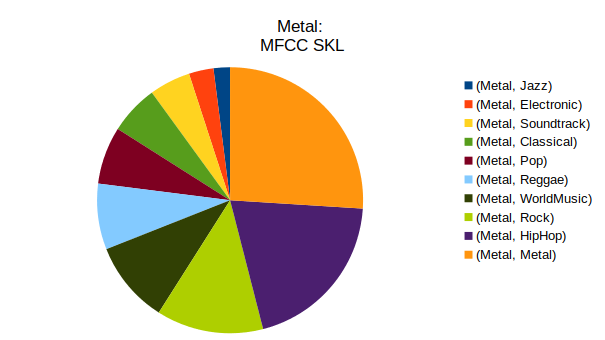
\includegraphics[scale=0.3]{Images/SparkFeat/Metal_MFCC_SKL.png}
				\caption{Metal MFCC SKL}
				\label{mms}
			\end{subfigure}%	
			
			\begin{subfigure}{.495\textwidth}
				\centering    
				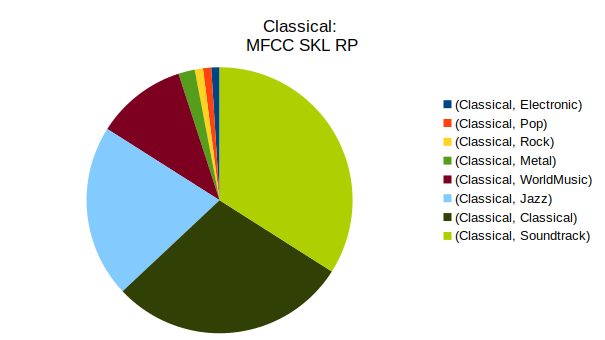
\includegraphics[scale=0.3]{Images/SparkFeat/Classical_MFCC_SKL_RP.png}
				\caption{Classical MFCC SKL RP}
				\label{cmsr}
			\end{subfigure}
			\begin{subfigure}{.495\textwidth}
				\centering     
				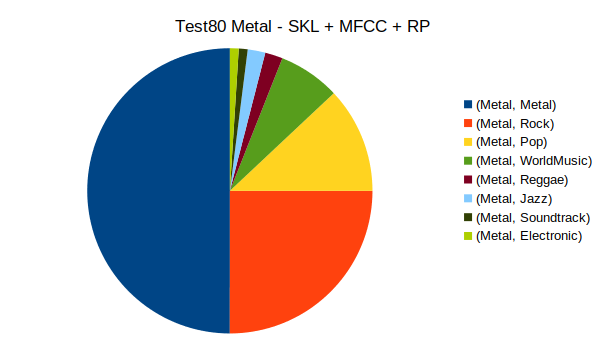
\includegraphics[scale=0.3]{Images/SparkFeat/Metal_MFCC_SKL_RP.png}
				\caption{Metal MFCC SKL RP}
				\label{mfsr}
			\end{subfigure}%		
	}}
	\caption{genre recall 100 songs}
	\label{fig:genrerec}
\end{figure}


\section{... and beyond genre boundaries}

\textit{\textbf{Rachmaninoff Prelude C\# minor full dataset Top 5 MFCC Euclidean\\}}
\\
\begin{itemize}
\item Songs/Klassik/Rachmaninoff-IdilBiret-Op3\_No2PreludeinC-SharpMinormp3
\item Jazz\&Klassik/100MeisterwerkederKlassik/Rachmaninov\_PianoConcertoNo2InCMinorOp18-1Moderato(Excerpt)mp3
\item Jazz\&Klassik/LangLang-Liszt/11\_LangLang\_PianoConcertoNo1inEflatmajorS124(LWH4)1Allegromaestosomp3
\item Jazz\&Klassik/PianoCollection/CD4-Brahms/03PianoSonataN°2inFsharpminorOp2-IIIScherzoallegrowav
\item Metal\&Rock/Compilations/RelapseSampler-RelapseSampler2015/SteveMoore-RelapseSampler2015-35Intro\&Creditsmp3
\item Jazz\&Klassik/LangLang-Liszt/12\_LangLang\_PianoConcertoNo1inEflatmajorS124(LWH4)2QuasiAdagio-Allegrettovivace-Allegroanimatomp3
\end{itemize}

\section{Improvements and outlook}

fma dataset\\
more state of the art similarity (blocked)\\
performance improvements\\

\section{Definition of similarity}
\textit{Rhythm, Timbre, Melodic, Genre and metadata, Genre specific features, combinations and variable model, Collaborative Filtering, Lyrics}

\textit{reduce hubness}

%\addtolength{\textheight}{-12cm}   % This command serves to balance the column lengths
% on the last page of the document manually. It shortens
% the textheight of the last page by a suitable amount.
% This command does not take effect until the next page
% so it should come on the page before the last. Make
% sure that you do not shorten the textheight too much.